\section{Auswertung}
\label{sec:Auswertung}
In Tab. \ref{tab:spektren} befindet sich die gemessene Photospannung bei varrierter Beschleunigungsspannung (bzw. Bremsspannung) für die Farbspektren Gelb, Grün und Violett.
\begin{table}
    \centering
    \csvreader[tabular=cc|,
    head=false,
    table head= $U_\text{gelb} \,/\, \si{\volt}$ & $I_\text{gelb} \,/\, \si{\nano \ampere}$\\
    \midrule,
    late after line= \\]
    {content/data/gelb.csv}{1=\eins, 2=\zwei}{$\num{\eins}$ & $\num{\zwei}$}
    \csvreader[tabular=cc|,
    head=false,
    table head= $U_\text{grün} \,/\, \si{\volt}$ & $I_\text{grün} \,/\, \si{\nano \ampere}$\\
    \midrule,
    late after line= \\]
    {content/data/gruen.csv}{1=\eins, 2=\zwei}{$\num{\eins}$ & $\num{\zwei}$}
    \csvreader[tabular=cc,
    head=false,
    table head= $U_\text{violett} \,/\, \si{\volt}$ & $I_\text{violett} \,/\, \si{\nano \ampere}$\\
    \midrule,
    late after line= \\]
    {content/data/violett.csv}{1=\eins, 2=\zwei}{$\num{\eins}$ & $\num{\zwei}$}
    \caption{Der gemessene Photostrom $I$ in Abhängigkeit der Spannung $U$ für drei verschiedene Farbspektren (gelb, grün, violett).}
    \label{tab:spektren}  
\end{table}
\\
Mithilfe einer linearen Ausgleichsrechnung der Form
\begin{equation}
  \sqrt{I} = a \cdot U + b
  \label{eqn:ausgleichsgerade}
\end{equation}
kann die Grenzspannung
\begin{equation}
  U_g = -\frac{b}{a}
\end{equation}
bestimmt werden:
\\
%ausgleichsgerade werte
\begin{align*}
  \text{Gelb:} && a &= \SI{7.2(16)e-06}{\frac{\sqrt{\ampere}}{\volt}} &\\
  && b &= \SI{9.9(19)e-05}{\sqrt{\ampere}} &\\
  && U_g &= \SI{-14(4)}{\volt}
\end{align*}
\\
\begin{align*}
  \text{Grün:} && a &= \SI{1.17(27)e-05}{\frac{\sqrt{\ampere}}{\volt}} &\\
  && b &= \SI{13.8(31)e-05}{\sqrt{\ampere}} &\\
  && U_g &= \SI{-12(4)}{\volt}
\end{align*}
\\
\begin{align*}
  \text{Violett:} && a &= \SI{1.93(31)e-05}{\frac{\sqrt{\ampere}}{\volt}} &\\
  && b &= \SI{18(4)e-05}{\sqrt{\ampere}} &\\
  && U_g &= \SI{-9.5(24)}{\volt}
\end{align*}
\\
In den Abb. \ref{fig:gelb}, \ref{fig:gruen}, \ref{fig:violett} ist die Wurzel des gemessenen Photostroms $\sqrt{I}$ gegen die angelegte Spannung $U$ aufgetragen.
Eine positive Spannung $U$ entspricht einer Beschleunigungsspannung.
Zudem ist die Ausgleichsgerade \eqref{eqn:ausgleichsgerade} eingezeichnet.

%figures
\begin{figure}
  \centering
  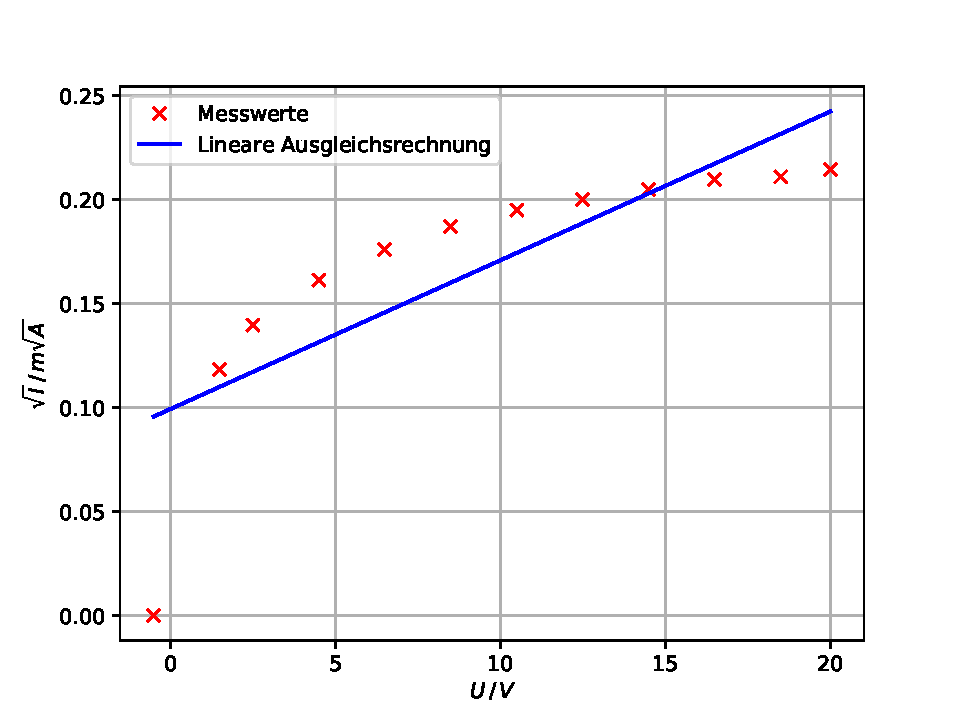
\includegraphics[width=0.8\textwidth]{content/data/gelb.pdf}
  \caption{Wurzel des Photostroms $\sqrt{I}$ in Abhängigkeit der Brems- bzw. Beschleunigungsspannung und eine Ausgleichsgerade für das gelbe Farbspektrum graphisch dargestellt. \cite{matplotlib}\cite{scipy}\cite{numpy}}
  \label{fig:gelb}
\end{figure}
\begin{figure}
  \centering
  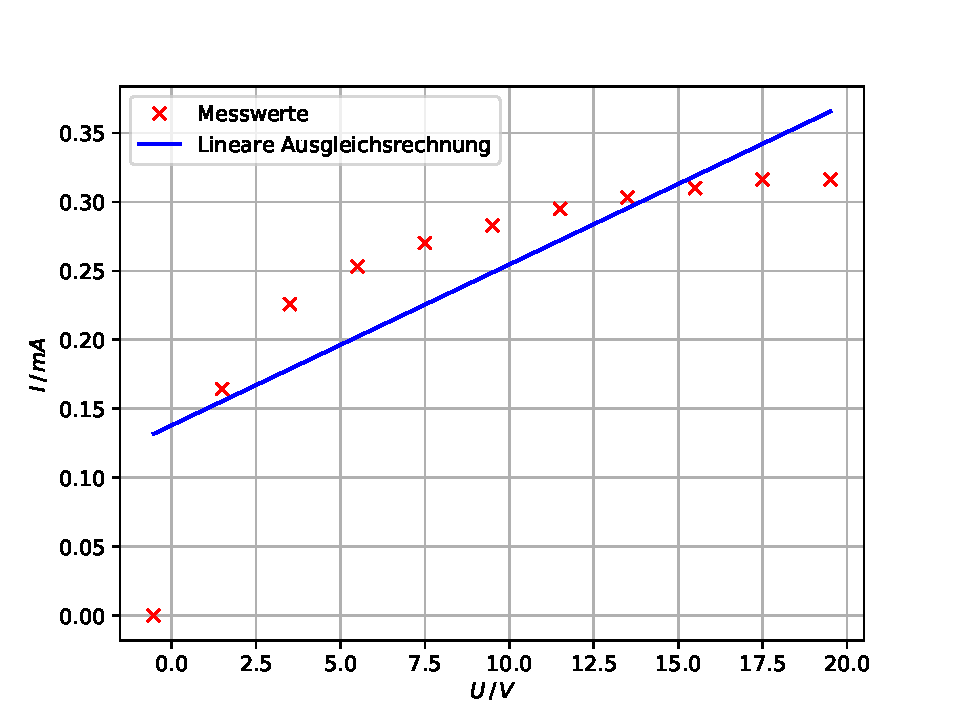
\includegraphics[width=0.8\textwidth]{content/data/gruen.pdf}
  \caption{Wurzel des Photostroms $\sqrt{I}$ in Abhängigkeit der Brems- bzw. Beschleunigungsspannung und eine Ausgleichsgerade für das grüne Farbspektrum graphisch dargestellt. \cite{matplotlib}\cite{scipy}\cite{numpy}}
  \label{fig:gruen}
\end{figure}
\begin{figure}
  \centering
  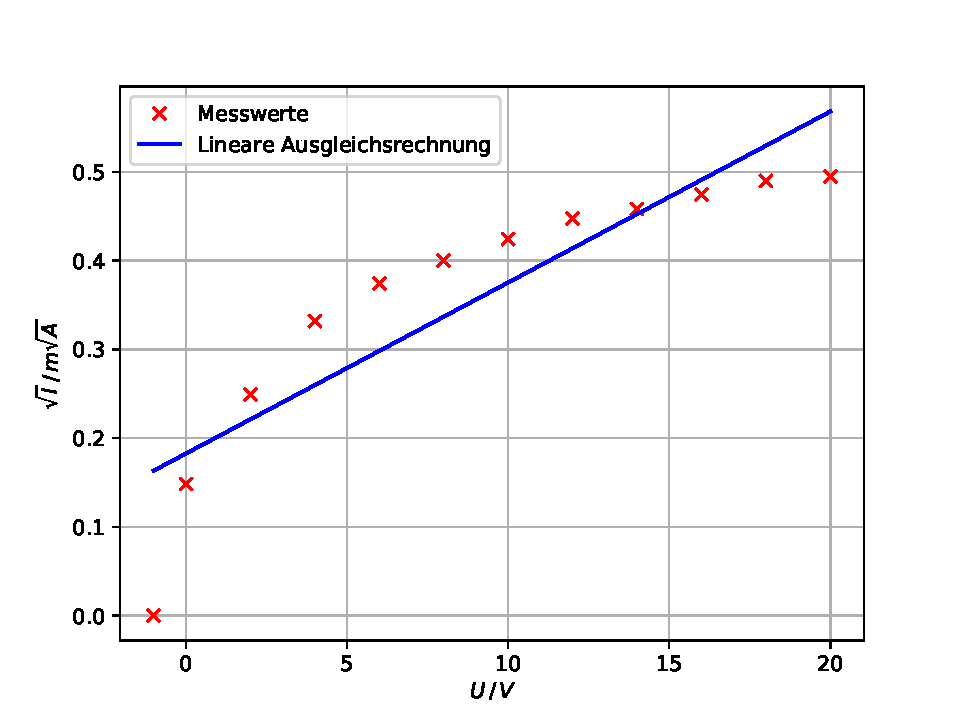
\includegraphics[width=0.8\textwidth]{content/data/violett.pdf}
  \caption{Wurzel des Photostroms $\sqrt{I}$ in Abhängigkeit der Brems- bzw. Beschleunigungsspannung und eine Ausgleichsgerade für das violette Farbspektrum graphisch dargestellt. \cite{matplotlib}\cite{scipy}\cite{numpy}}
  \label{fig:violett}
\end{figure}

Als nächstes wird der Zusammenhang der Grenzspannungen $U_g$ der einzelnen Farbspektren und die Frequenz $\nu = \frac{c}{\lambda}$ untersucht.
Die Frequenz der einzelnen Farbspektren \cite[9]{anleitung} entnommen.
Konstanten wie die Lichtgeschwindigkeit $c$ und das planksche Wirkungsquantum $h$ werden der Literatur \cite{konstanten} entnommen.
In Tab. \ref{tab:grenzspannung} befinden sich die durch die Ausgleichsrechnung bestimmenten Grenzspannungen.
\begin{table}
  \centering
  \begin{tabular}{c|ccc}
    \toprule
    Farbspektrum & $\lambda \,/\, \si{\nano\metre}$ & $\nu \,/\, \si{\tera\hertz}$ & $U_g \,/\, \si{\volt}$ \\
    \midrule
    Gelb & $577$ & $519.57$ & $\SI{-14(4)}{}$ \\
    Grün & $546$ & $549.07$ & $\SI{-12(4)}{}$ \\
    Violett & $434$ & $690.77$ & $\SI{-9.5(24)}{}$ \\
    \bottomrule
  \end{tabular}
  \caption{Grenzspannung $U_g$ verschiedener Farbspektren mit Wellenlänge $\lambda$ und Frequenz $\nu$ aufgelistet.}
  \label{tab:grenzspannung}
\end{table}
Eine lineare Ausgleichsrechnung
\begin{equation*}
  U_g = \nu \cdot \frac{h}{e_0} - \frac{A_k}{e_0}
\end{equation*}
ergibt folgende Parameter:
\begin{align*}
  \frac{h}{e_0} &= \SI{2.3(6)e-14}{\frac{\joule}{\ampere}} \\
  A_k &= \SI{25.4(35)}{\electronvolt}
\end{align*}
Die lineare Ausgleichsrechnung und die zugehörigen Messwerte sind in Abb. \ref{fig:grenzspannung} graphisch dargestellt.
\begin{figure}
  \centering
  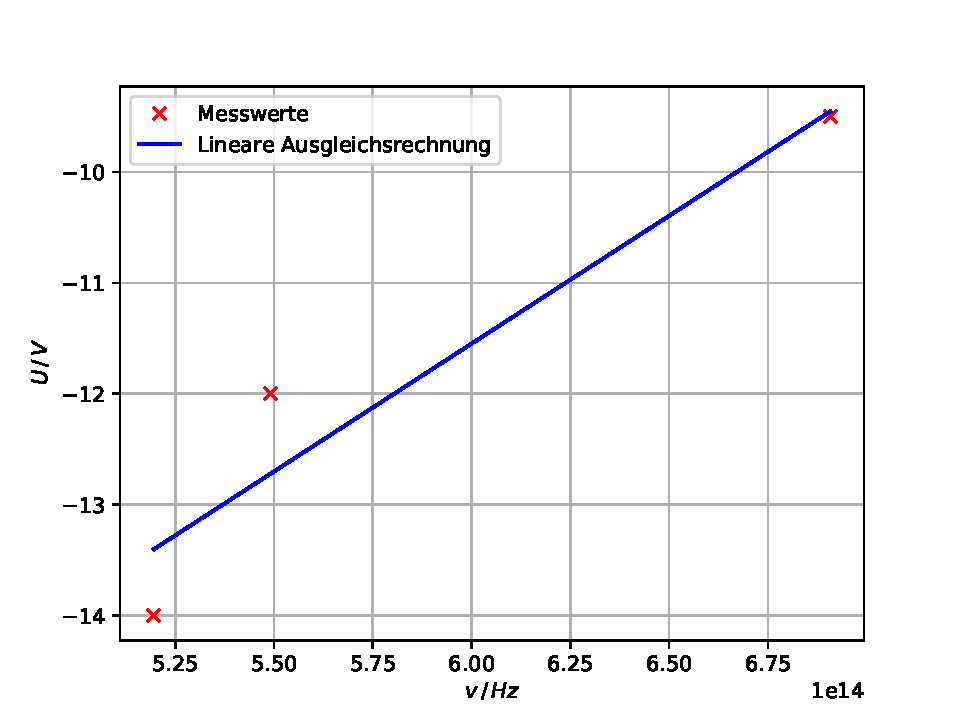
\includegraphics[width=0.8\textwidth]{content/data/grenzspannung_ausgleich.pdf}
  \caption{Messwerte und eine lineare Ausgleichsgerade der Messwerte graphisch dargestellt. \cite{matplotlib}\cite{scipy}\cite{numpy}\cite{uncertainties}}
  \label{fig:grenzspannung}
\end{figure}
\\
Der erste Messwert $U$ jedes Farbspektrums entspricht der experimentell bestimmten Grenzspannung $U_{g,2}$.
Die Spannung wird zuerst so varriert, dass kein Photostrom gemessen wird (1. Messwert) und dann in konstanten Schritten erhöht.
Eine lineare Ausgleichsrechnung mit $U_{g,2} = 1. \text{ Messwert}$ (siehe Tab. \ref{tab:grenzspannung_2}) ergibt folgende Parameter:
\begin{align*}
  \frac{h}{e_0} &= \SI{-3.05(33)e-15}{\frac{\joule}{\ampere}} \\
  A_k &= \SI{1.11(20)}{\electronvolt}
\end{align*}

\begin{table}
  \centering
  \begin{tabular}{c|ccc}
    \toprule
    Farbspektrum & $\lambda \,/\, \si{\nano\metre}$ & $\nu \,/\, \si{\tera\hertz}$ & $U_{g,2} \,/\, \si{\volt}$ \\
    \midrule
    Gelb & $577$ & $519.57$ & $-0.50$ \\
    Grün & $546$ & $549.07$ & $-0.53$ \\
    Violett & $434$ & $690.77$ & $-1.00$ \\
    \bottomrule
  \end{tabular}
  \caption{Grenzspannung $U_{g,2}$ verschiedener Farbspektren mit Wellenlänge $\lambda$ und Frequenz $\nu$ aufgelistet.}
  \label{tab:grenzspannung_2}
\end{table}
Die lineare Ausgleichsrechnung ist in Abb. \ref{fig:grenzspannung_2} zu sehen.
\begin{figure}
  \centering
  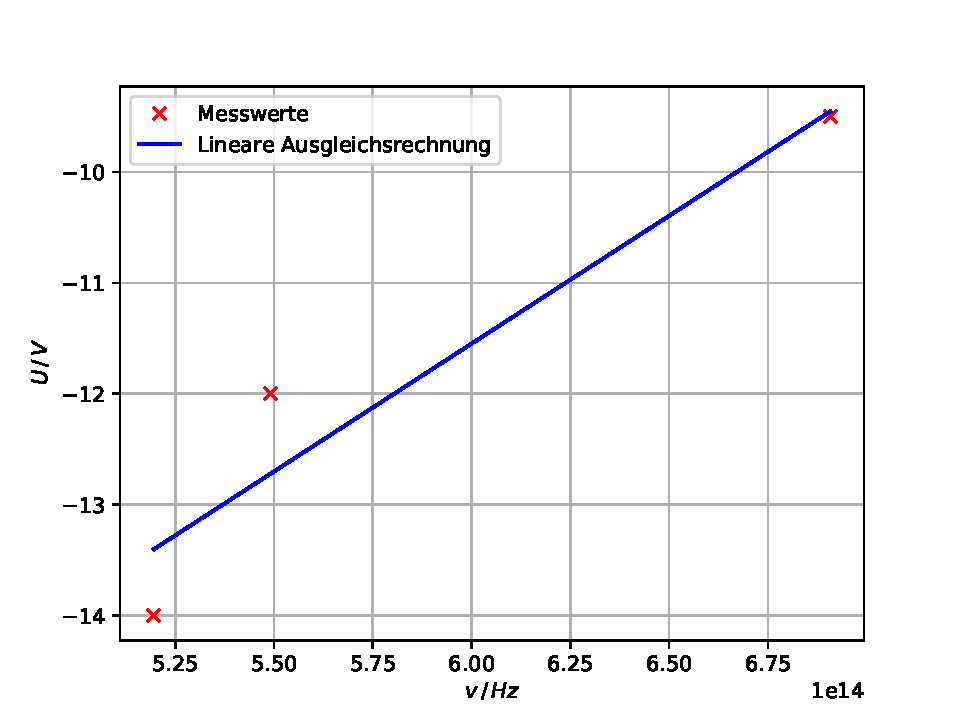
\includegraphics[width=0.8\textwidth]{content/data/grenzspannung_ausgleich.pdf}
  \caption{Messwerte und eine lineare Ausgleichsgerade der Messwerte graphisch dargestellt. \cite{matplotlib}\cite{scipy}\cite{numpy}\cite{uncertainties}}
  \label{fig:grenzspannung_2}
\end{figure}
Der Literaturwert \cite{konstanten} liegt bei
\begin{equation*}
  \frac{h}{e_0} = \SI{-4.14e-15}{\frac{\joule}{\ampere}} \,.
\end{equation*}
